% !TeX spellcheck = en_US

\chapter{Evaluation}
\section{Qualitative Evaluation on Real-World Datasets}
\label{sec:EvaluationOnDatasets} % Now, we can use "\autoref{sec:<my-label>}" to refer to this chapter
The face segmentation network was tested on two different datasets with real-life images: Firstly with the Caltech Occluded Faces in the Wild (COFW) dataset by \cite{cofw} and secondly with the parts-labeled LFW dataset of the University of Massachusetts \cite{LFW_dataset}. Both datasets are designed to present faces in real-world conditions. The COFW dataset provides 29 landmarks and a bounding box for all 507 images. The original LFW dataset contains 13'000 images of 1'680 different subjects. Each face is labeled with the name of the depicted person. This database is actually meant to test facial recognition/verification algorithms. Nevertheless, we tested the segmentation of the FCN on the 500 images of the Parts-LFW validation set. For each image, there is a ground truth segmentation, which makes it possible to measure the quality of the FCN's segmentation in numbers.
\\
\subsection{Evaluation on the COFW Dataset}
Since on the COFW dataset only landmarks and bounding-boxes are given, the segmentation had to be evaluated qualitatively. We tried reconstructing the graphic on Nirkins \cite{nirkin2018_faceswap} github-repository 'face\_segmentation' [\Cref{fig:chap2:myMatrix}]. In  [\Cref{fig:chap2:myMatrix_EGGER}] the same 18 images are segmented by the iterative method of Egger et al. This algorithm outputs both, parameters for a 3DMM and a segmentation. [\Cref{fig:chap2:COFW_Fits}] shows the fits of 9 images of the COFW dataset where both segmentations are used. A matrix of the other 9 fits can be found in the Appendix [\Cref{appendix:COFW}].

\begin{figure}[H]
	\centering
	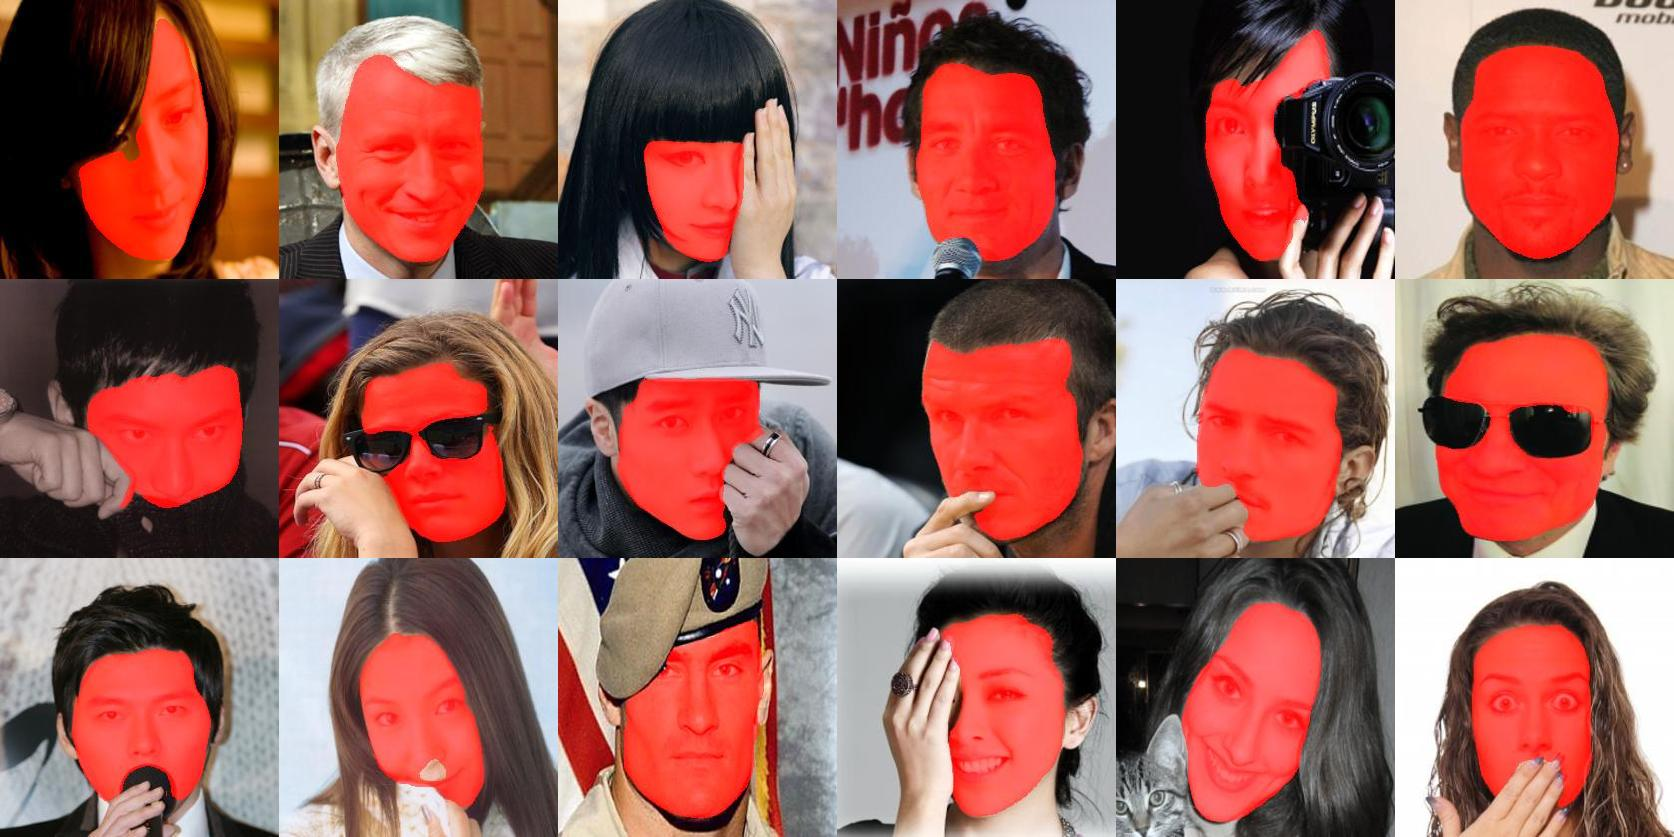
\includegraphics[width=0.9\textwidth]{Figures/chap2/myMatrix.jpg}
	\caption{18 images of the COFW Dataset overlaid with the FCN output (in red). The segmentation results are very similar to those on \href{https://github.com/YuvalNirkin/face_segmentation}{Nirkin's github page}.}
	\label{fig:chap2:myMatrix}
\end{figure}

\begin{figure}[H]
	\centering
	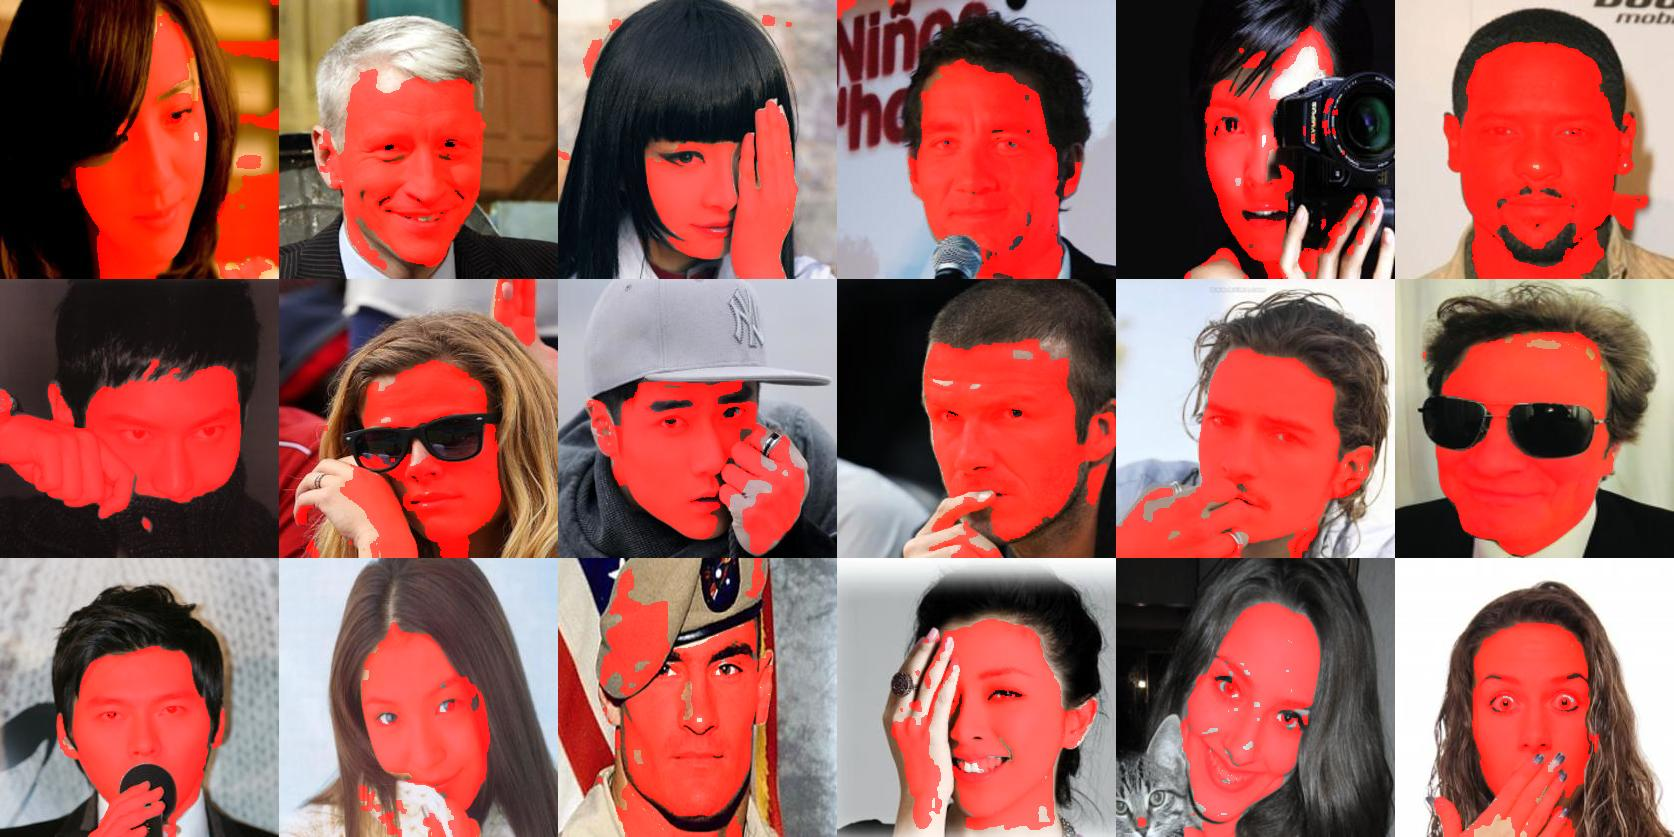
\includegraphics[width=0.9\textwidth]{Figures/chap2/myMatrix_EGGER.jpg}
	\caption{The same target images as in [Figure \ref{fig:chap2:myMatrix}], but this time with the (final) segmentation of the occlusion-aware method of Egger et al \cite{egger_paper}. Often the eyes are not segmented or the segmentation includes skin other than the face (eg. hands).}
	\label{fig:chap2:myMatrix_EGGER}
\end{figure}

\begin{figure}[H]
	\centering
	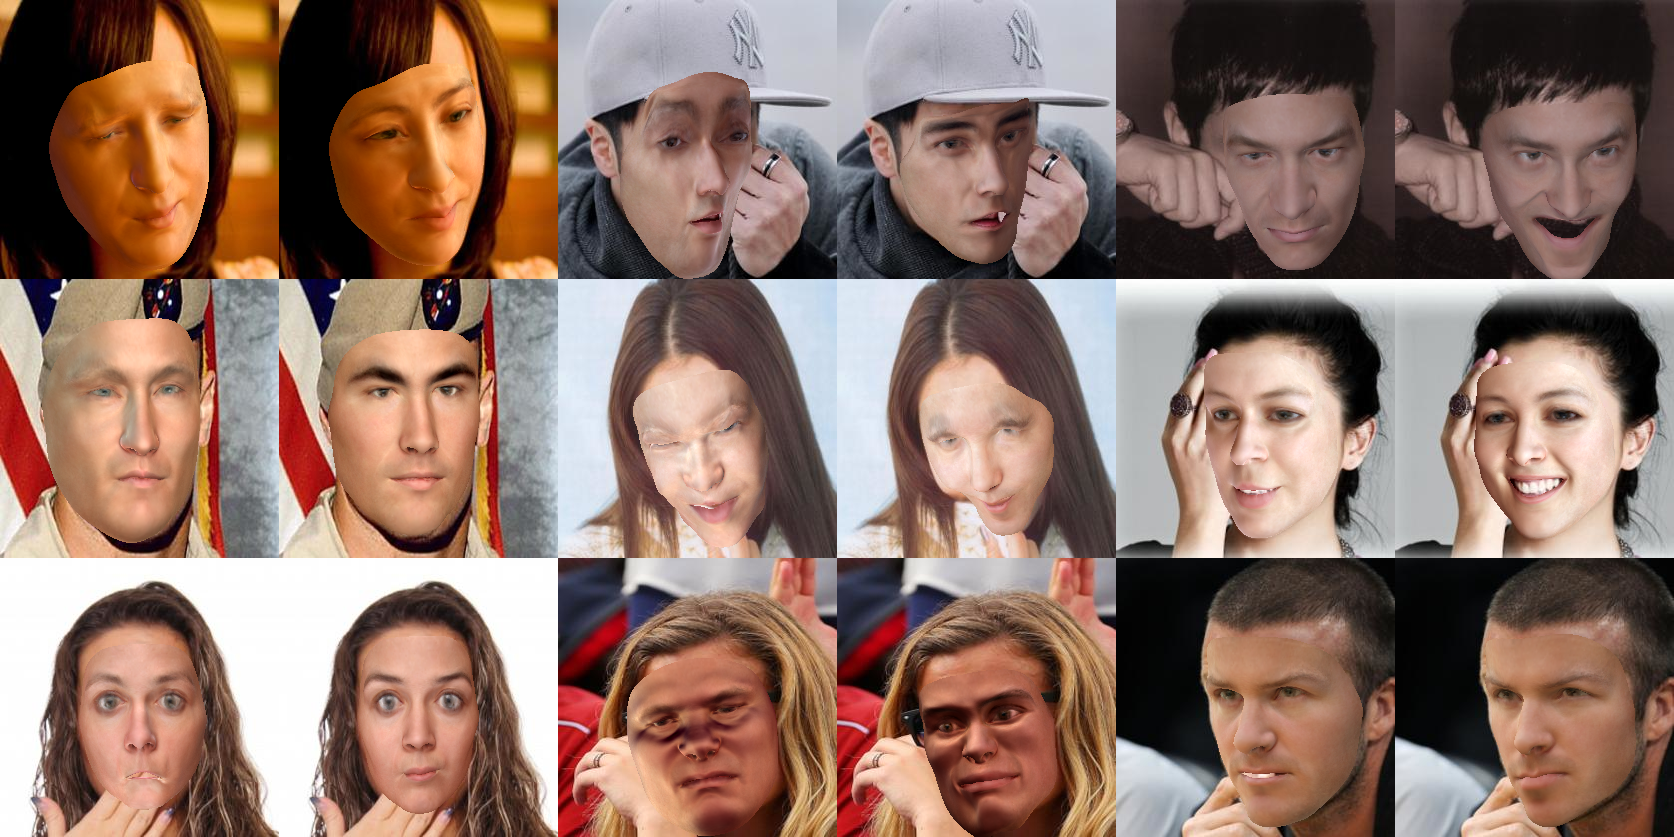
\includegraphics[width=0.9\textwidth]{Figures/chap2/COFW_Fits.png}
	\caption{Tuples of facial images. In every tuple, the first image shows the fit with the mask of the algorithm of Egger et al itself [Figure \ref{fig:chap2:myMatrix_EGGER}]. The second shows the fit with the FCN mask which are depicted in [Figure \ref{fig:chap2:myMatrix}].}
	\label{fig:chap2:COFW_Fits}
\end{figure}

\subsection{Evaluation on the Parts-LFW Dataset}
In the Parts-LFW dataset, we had a ground-truth mask for every image. The mask distinguishes between hair, skin, and background. We looped through all the provided ground-truth masks and overlaid them with the segmentations of the FCN. Now we can compare the labels of both masks. The evaluation is quite impressive. The FCN performs very well in segmenting only pixels that belong to the face. On average over the 500 images of the Parts-LFW dataset, there are $98.5\%$ right non-segmentations (only 1.5\% false positives). On the other hand, only $85.4\%$ of all the pixels which belong to the face are segmented as face (14.6\% false negatives) which is not a good but acceptable result. [Figures \ref{fig:drew:sf1} and \ref{fig:drew:sf2}] depict such a face image and its mask. Unfortunately, on the given mask no distinction is made between face and other parts of the body, but everything is segmented as skin [Sub-figures \ref{fig:drew:sf1} and \ref{fig:drew:sf2}]. However, it is more problematic that some faces have beards. The FCN of \cite{nirkin2018_faceswap} segments facial hair which was excluded from the provided labels. Therefore, we had to manually remove these images [Sub-figures \ref{fig:ali:sf3} and \ref{fig:ali:sf4}]. To reduce the effort, we took the Parts-LFW validation set containing 500 images. After removing the ones with a beard or mustache, we were left with 447 images. The results are summarised in [\Cref{fig:Parts-LFW}].

\begin{figure}[H]
	\centering
	\subbottom[A facial-image with the segmentation of the FCN highlighted in red.]{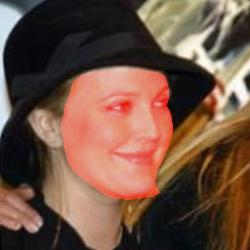
\includegraphics[width=0.4\textwidth]{Figures/chap2/drew/drew_original.jpg}\label{fig:drew:sf1}}
	\subbottom[The provided ground-truth segmentation of the image \ref{fig:drew:sf1} overlaid with the mask of the FCN (red).]{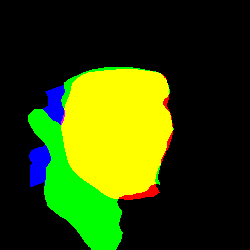
\includegraphics[width=0.4\textwidth]{Figures/chap2/drew/drew_segments.png}\label{fig:drew:sf2}}
	
	
	\subbottom[An facial-image with the segmentation of the FCN highlited in red.]{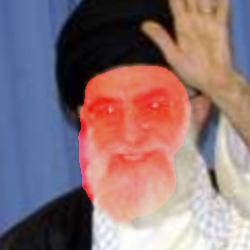
\includegraphics[width=0.4\textwidth]{Figures/chap2/ali/ali_original.jpg}\label{fig:ali:sf3}}
	\subbottom[The provided ground-truth segmentation of the image \ref{fig:ali:sf3} overlaid with the mask of the FCN (red).]{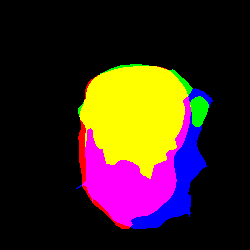
\includegraphics[width=0.4\textwidth]{Figures/chap2/ali/ali_segments.png}\label{fig:ali:sf4}}
	\caption{In each row, the left-hand is an image of the Parts-LFW dataset overlaid with the segmentation of the FCN (red). The skin region is colored in green, hair regions are blue, and the background is black. The mixed colours (yellow and magenta) arise because the red mask of the FCN is also present in these plots.}
	\label{fig:tm}
\end{figure}

\begin{figure}
\begin{center}
\begin{tabular}{l|l} \hline
	false-positives (hair) & 7.04\%\\ \hline
	false-positives (background) & 0.68\%\\ \hline
	false-negatives (background) & 14.13\%\\ \hline
	right-segmentations & 85.87\%\\ \hline
	right non-sementations & 99.32\% \\ \hline
\end{tabular}
\end{center}
\caption{The averages over the 447 images of the Parts-LFW evaluation set of \cite{LFW_dataset}. The FCN recognises (almost) only pixels which belong to the face (little false positives). By reducing from 500 to 447 images, we were able to lower this number even more. Unfortunately, there are many false negatives (skin pixels labeled as background).} 
\label{fig:Parts-LFW}
\end{figure}
%\vspace{.5cm}

\FloatBarrier

\section{Evaluation on Synthetic-Data}
\subsection{Experimental Setup}
In order to evaluate the FCN on synthetic-data, we used the parametric face image generator of Kortylewski et al \cite{parametric} to produce images of a random face in a given pose [\Cref{fig:syntheticData_samples}]. We extended the software so that it now renders occlusions over the face. Furthermore, we changed the parametric face image generator so that it now generates a ground-truth mask, which classifies every pixel either as part of the face or as non-face. In this experiment the estimated mask of the FCN is compared to the ground-truth mask of the parametric face image generator.

\begin{figure}[H]
	\centering
	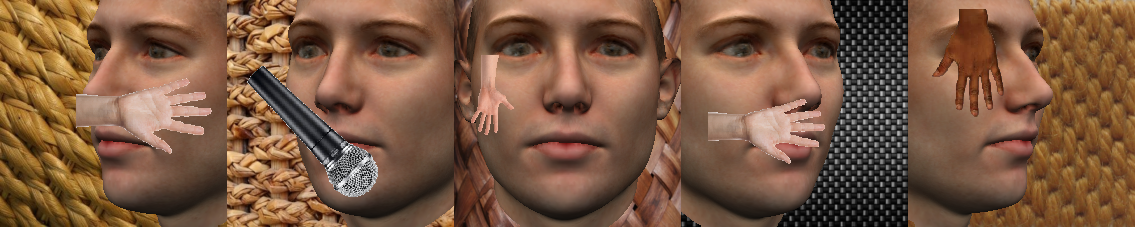
\includegraphics[width=\textwidth]{Figures/chap2/syntheticData_samples.png}
	\caption{Five examples of the synthetic face images. The same face is shown with yaw angles $-45$\textdegree, $-25$\textdegree, $0$\textdegree, $25$\textdegree, and $45$\textdegree. The type of the occlusion is chosen randomly and in an arbitrary orientation and position.}
	\label{fig:syntheticData_samples}
\end{figure}

\subsection{Data for the Experiment}
Nirkin et al \cite{nirkin2018_faceswap} claim that both the face itself and the context of the face play an important role for the outcome of the segmentation. To prevent this effect and reduce the impact of outliers, we repeat the experiment 5 times with a different face and a different background image. The number of images used in a single run of the experiment varies but is similar to the number of grid cells in the following plots that visualise the experiments: 101 images were used to measure the dependence of one rotation alone (top row of [\Cref{fig:evaluation_angles}]), in the bottom row of [\Cref{fig:evaluation_angles}] 441 images were used, to plot the rotations versus the degree of occlusion [\Cref{fig:occVal40}] we used 340 images per plot and 380 were used for the plots in [\Cref{fig:occVal90}].


\subsection{Dependence of the Euler Angles}
Because we are now able to create synthetic face images in any desired pose, we first want to measure the segmentation-accuracy of the FCN for the rotations: Yaw, roll, and pitch. We evaluate each rotation itself and every possible combination of two rotations in order to create a hierarchy under the rotations [\Cref{fig:evaluation_angles}].\\

\begin{figure}[H]
	\centering
	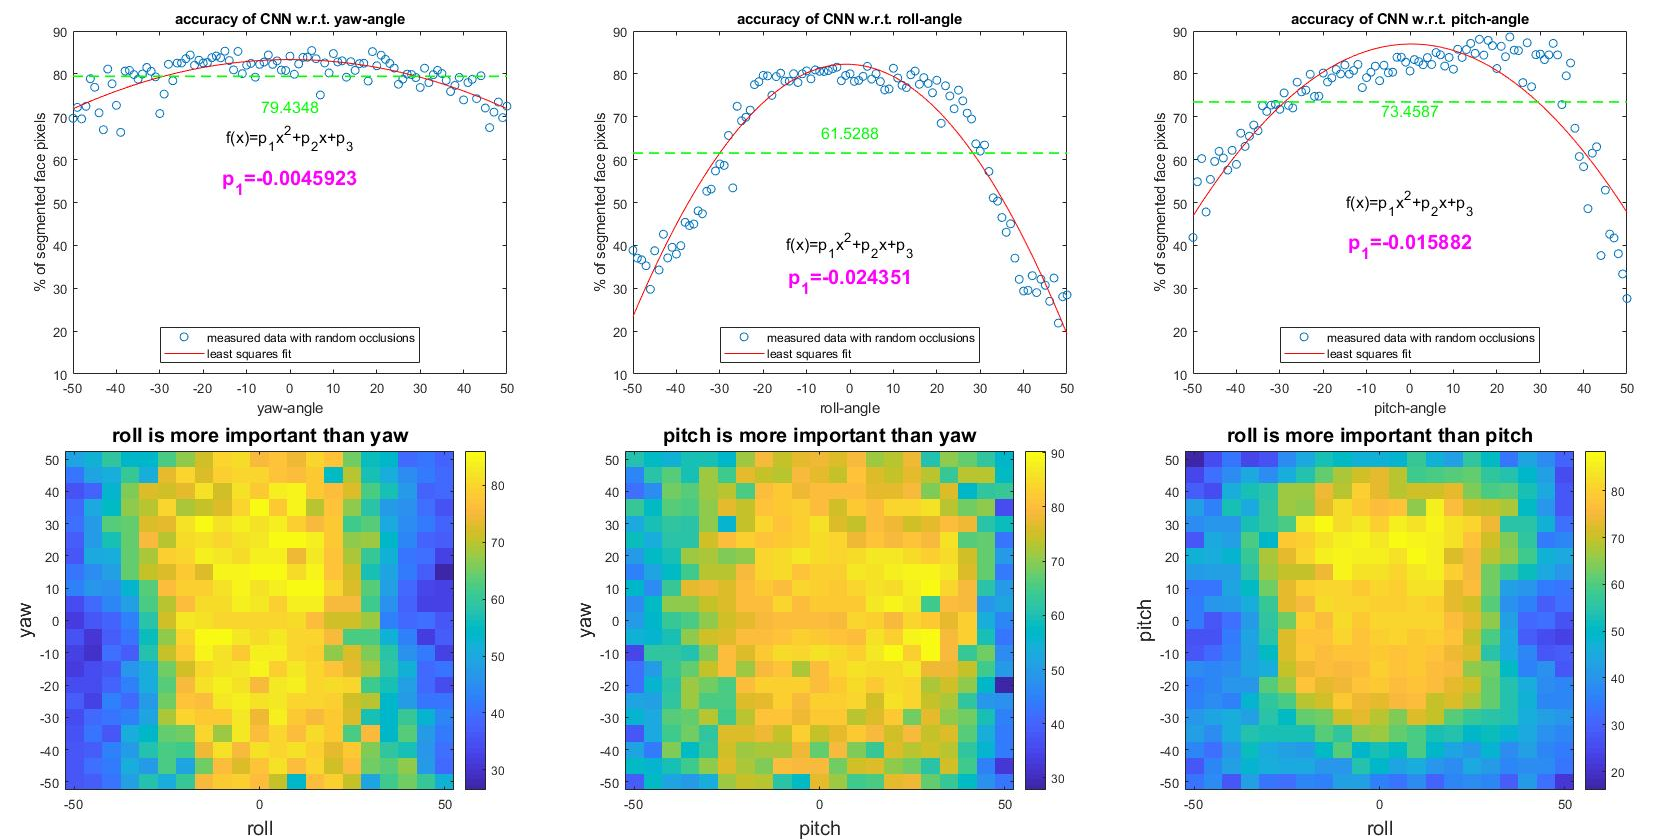
\includegraphics[width=\textwidth]{Figures/evaluation_angles.png}
	\caption{In the plots on the top row we see the segmentation accuracy in percent (on the y-axis) for every single image (with face angles from $-50$\textdegree to $50$\textdegree on the x-axis). The point cloud is approximated by a quadratic function via a least squares fit (red curve / $f(x)$). The first parameter of this function determines the opening angle ($p_1$). The greater the absolute value of this parameter, the more sensitive is the FCN to the respective rotation. In the bottom row, the colours indicate the segmentation accuracy. The brighter the colour, the better the segmentation. In every plot, there is a cluster of high accuracy segmentations centered in the origin. The rotation on whose axis the cluster has the lower variance is the more important of the two. A rotation is called 'important' when a small change of this rotation leads to a failure of the FCN.}
	\label{fig:evaluation_angles}
\end{figure}

From the graphs of [\Cref{fig:evaluation_angles}], we can conclude that the roll rotation is the most relevant for the FCN, that the pitch rotation is less important, and that the accuracy of the FCN is still good even with high yaw angles (yaw is the least important rotation). 

\subsection{Random Boxes as Occlusions}
The 340 images for the plots in [\Cref{fig:occVal40}] consist of pictures with 20 different occlusion levels, where one rotation is in the range from $-40$\textdegree to $40$\textdegree and the other two rotations are set to $0$.\\
\\
In the given table of [\Cref{fig:angle_table}], all provided images show a face, from which 20\% of the pixels are occluded by a randomly colored box. We can optically verify, that firstly, a high yaw rotation, despite the occluding box, has not much of an effect. Secondly, that in both situations, $-40$\textdegree and $40$\textdegree of the roll rotation, the result is not satisfying. That is interesting because no matter how big the roll rotation is, the information (the face) stays the same. Further, in the third column, the segmentation with a negative pitch angle is much worse than with a positive one. This supports our assumption that the roll rotation plays a big role, followed by the (asymmetric) pitch rotation. The yaw rotation is less important because even at large angles a big part of the face is still segmented.

% The source for this table was this post: https://stackoverflow.com/questions/2771856/centering-text-horizontally-and-vertically-in-latex
% To add padding for the cell contents: https://tex.stackexchange.com/questions/31672/column-and-row-padding-in-tables
\begin{figure}[H]
	\begin{center}
		\newcolumntype{C}{>{\centering\arraybackslash} m{2cm} }  %# New column type
		\begin{tabular}{m{1cm}|SC|SC|SC}
			& yaw & roll & pitch\\ \hline
			-40 & \subfloat{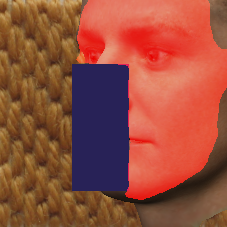
\includegraphics[width=0.1\textwidth]{Figures/-40_0_0_occVal_20.png}} &
			\subfloat{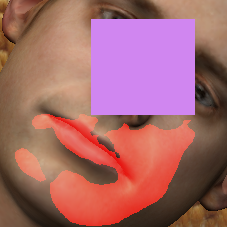
\includegraphics[width=0.1\textwidth]{Figures/0_0_-40_occVal_20.png}} &
			\subfloat{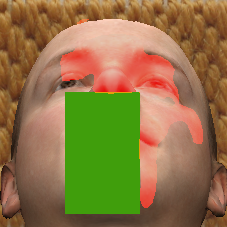
\includegraphics[width=0.1\textwidth]{Figures/0_-40_0_occVal_20.png}} \\ \hline
			40 & \subfloat{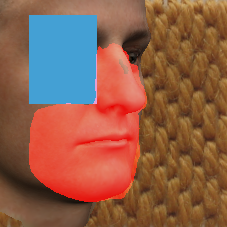
\includegraphics[width=0.1\textwidth]{Figures/40_0_0_occVal_20.png}} &
			\subfloat{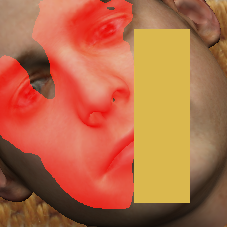
\includegraphics[width=0.1\textwidth]{Figures/0_0_40_occVal_20.png}} &
			\subfloat{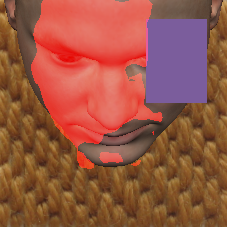
\includegraphics[width=0.1\textwidth]{Figures/0_40_0_occVal_20.png}} \\
		\end{tabular}
	\end{center}
	\caption{Based on these images, we can see that the roll rotation is the most sensitive, followed by the pitch rotation, where the segmentation works better on positive angles than on negative ones. The most stable detection is at the yaw rotation. It has the least influence on the segmentation.}
	\label{fig:angle_table}
\end{figure}

\begin{figure}[H]
	\centering
	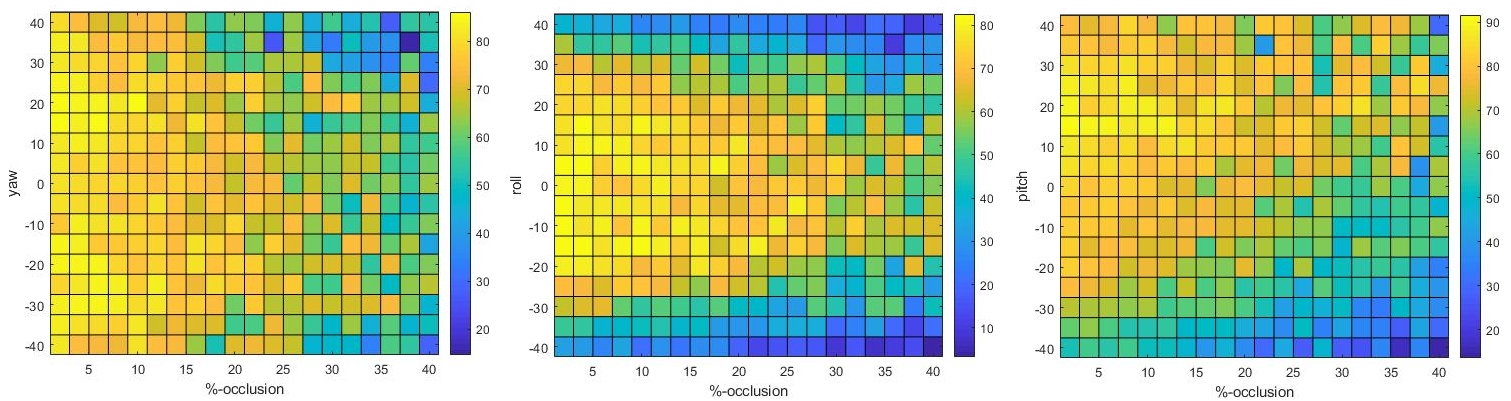
\includegraphics[width=\textwidth]{Figures/occVal_angles.png}
	\caption{The colour of each grid cell indicates the accuracy of the segmentation of the FCN on a set of faces turned by the corresponding angle and occluded with a rectangle so that the corresponding amount (on the x-axis) of the face is hidden. The brighter the colour, the better the segmentation. On each plot, we would expect to see a triangle pointing to the right. This means that the combination of a large angle and a big occlusion make the face even more unsegmentable.}
	\label{fig:occVal40}
\end{figure}

\pagebreak
 
We see that the segmentation is very sensitive to the roll rotation and that the FCN is not trained to segment faces that are aslope. Surprisingly, the yaw rotation plays a subordinate role here. The rightmost plot of [\Cref{fig:occVal40}] tells us, that the sign of the pitch rotation plays a significant role because the plot is asymmetric. Since we are not able to determine at which angles exactly the FCN begins to fail, we repeated the experiment with a higher angle range [\Cref{fig:occVal90}].

\begin{figure}[H]
	\centering
	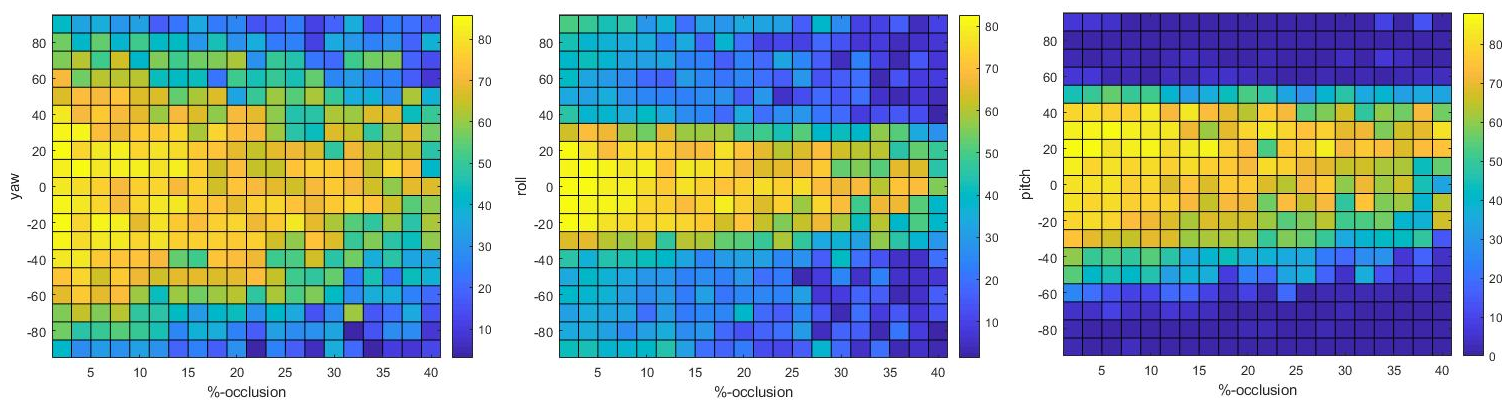
\includegraphics[width=\textwidth]{Figures/occVal_angles_90.png}
	\caption{This plot shows the outcome of a similar experiment as shown in Figure \ref{fig:occVal40} with less resolution. All the angles (yaw, pitch, and roll) range from $-90$\textdegree to $90$ \textdegree in steps of 10\textdegree. The scale on the "\%-occlusion" stays the same as in Figure \ref{fig:occVal40}. We can clearly see the limits of the FCN even with a occlusion of 2\%. Very interesting is the hard transition from good segmentations to bad segmentations in the two right plots.}
	\label{fig:occVal90}
\end{figure}



Although in practice exact rectangles are very rare, boxes as occlusions are very simple and we are in control of the rectangle's size. It is the simplest method to occlude a given amount of the face region.